\chapter{Afinal, o que é um robô?}
\section*{Introdução}
O desejo de solucionar problemas do dia-a-dia de maneira mais eficiente e simples, foi - e ainda é - um dos maiores promotores para o desenvolvimento tecnológico das mais diversas sociedades. De acordo com a necessidade de cada período, cientistas (engenheiros, matemáticos, físicos, etc) de diferentes povos propunham maquinários e ferramentas que pudessem operar em conjunto com outros seres vivos para \textbf{modificar} a forma de trabalho, melhorando a qualidade de vida dos trabalhadores e das suas famílias. Com isso, impulsionou-se a busca por maiores níveis de \textbf{automação}, consequentemente levando às tentativas de aplicar esse conceito no cotidiano, sendo esse o patamar que alcançamos e presenciamos nos dias atuais. \par
É nesse contexto que a ideia da utilização de robôs para a realização de diversas tarefas acabou se popularizando, colocar uma máquina para completar uma tarefa muito trabalhosa ou difícil e assim poupar trabalho humano é um dos focos da robótica. O robozinho utilizado como material de estudo no nosso curso é o \textit{Sparki}, ele é uma dessas máquinas que tem como objetivo facilitar a nossa vida, nesse caso o ensino de programação, mas o que difere ele e outros robôs de um ar condicionado ou um projetor?



\section{Para que estudar a definição de robô?}
Como descrito na introdução desse capítulo, a robótica está presente em diversos aspectos do nosso cotidiano. Dentre as mais diversas aplicações existentes, podemos listar algumas:


- Culinária, robôs que auxiliam na preparação de pratos e na entrega dos mesmos em restaurantes (segue-linha)

- Robôs industriais, como carregados (segue-linha), robôs montadores de peças em indústrias

- Robôs cirúrgicos, como o Star (), o PRECEYES (áreas delicadas, como os olhos), CorPath (operações cirúrgicas a distância através do Wifi), The Monarch Platform (broncoscopia, i.e. intervenção cirúrgica nos brônquios), Mako Rio (auxiliar em implante em joelhos e costela), Versius (cirurgias não invasivas).

- Robôs para comunicação com criança

- Robôs de exploração espacial, como o Hover em Marte

- Robô para inspecionar de tubulações.

- Robô para serviços de casa (seja de superfícies aquáticas, ou terrestres). Exemplos: Row-bot, Ro-Boat, Roomba

    \begin{figure}[h]
    \caption{Exemplo de um robô, o Roomba}
     
    \centering 
    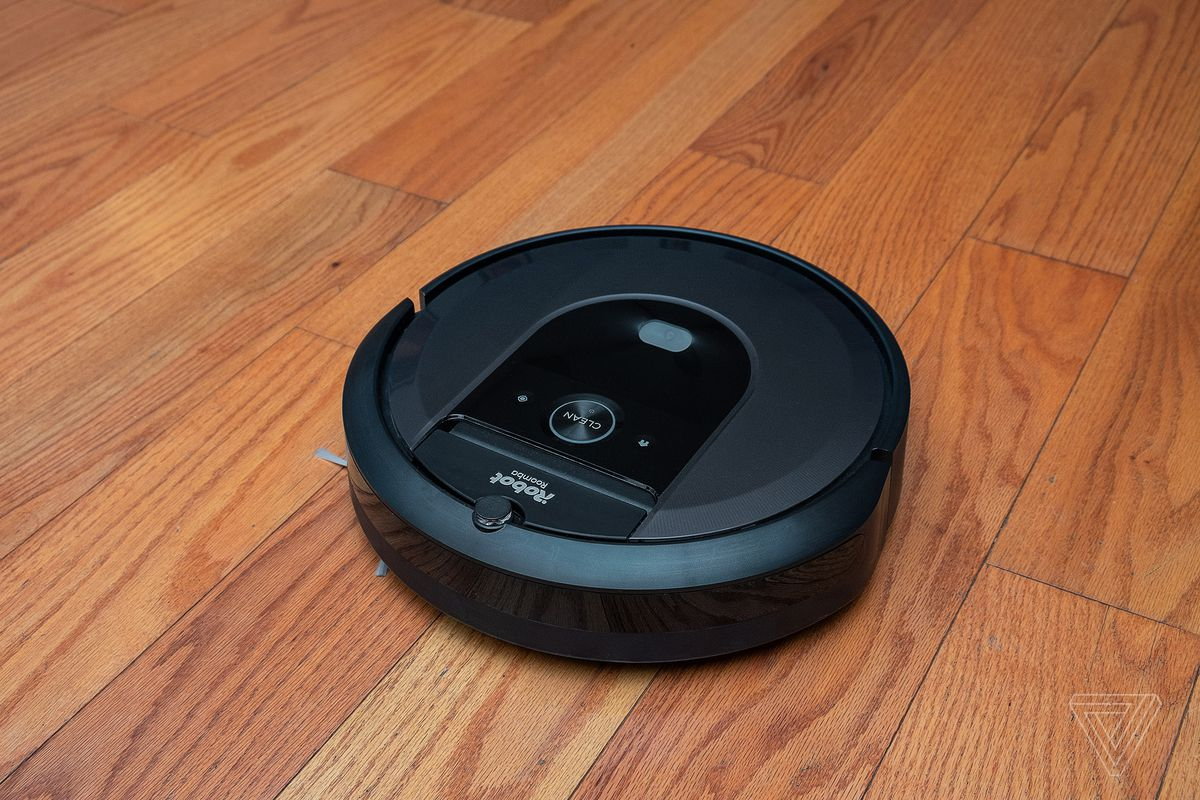
\includegraphics[width=8cm]{Figuras/roomba.jpg}
    \label{figura:roomba.jpeg}
    \end{figure}
 

\section{Definindo um robô}
Para uma máquina ser considerada um robô, a primeira coisa que ela deve ser capaz de fazer é raciocinar de alguma maneira.

\textit{Como assim, um robô tem que ser capaz de pensar assim como nós pessoas?}

Não necessariamente, algo assim é muito complexo e difícil de acontecer... quando dizemos que um robô deve raciocinar, queremos dizer que ele deve ter a capacidade de analisar o mundo ao seu redor e tomar decisões a partir do que ele analisou, ele precisa agir em função do seu ambiente. Um robô segue linhas por exemplo, necessita de algum sensor que permita a ele encontrar a localização da linha e a partir dai decidir como irá se movimentar sobre ela e o que fazer caso perca a linha de vista. De maneira geral, a ação realizada pelos robôs normalmente é algum tipo de movimento, alguma atividade mecânica como andar ou mover algo, um semáforo que acende a luz vermelha para os carros para possibilitar a passagem de pedestres após ter seu botão apertado não é considerado um robô, uma porta automática de um shopping se aproximaria mais do que é um robô.


\textit{Qual a relevância deste assunto no mundo? Afinal, para que diabos estou lendo esta apostila? Eu sei que eu vou ganhar um diploma do curso, mas... E aí? O que mais que isso aqui pode me acrescentar?}

Nosso curso busca ajudar os alunos a entender de forma simples como que um robô, um computador ou outros equipamentos raciocinam, como que nós pessoas somos capazes de criar linhas de pensamento para coisas não pensantes. Nós mostraremos que a programação não é um bicho de sete cabeças e forneceremos a base necessária para que vocês cheguem mais preparados e entusiasmados em algum curso superior, técnico ou trabalho que aborde programação.


\vfill
\begin{center}

    \textbf{Definição}
    
    \justify
    Um robô é uma máquina \textbf{autônoma}, que existe no \textbf{mundo físico}, possui \textbf{sensores} para perceber o ambiente e consegue \textbf{agir} sobre o meio para alcançar um ou mais objetivos definidos.
\end{center}

Nós já falamos sobre os sensores e conseguir agir sobre o meio, mas e os outros requisitos?

Existir no mundo físico nada mais é do que algo que somos capazes de tocar e manipular, uma bola de futebol por exemplo existe no mundo físico, os sonhos que temos ao dormir não existem no mundo físico, pois não somos capazes de tocá-lo.

Uma máquina autônoma ou automática, é uma máquina que após ligada ela funciona sozinha sem a constante necessidade de interferência externa, ela ainda pode requer o aperto de botões ou o recebimento de outros tipos de comandos, mas a ideia é que ela seja capaz de realizar tarefas sozinha quando for necessário.

\section*{Para saber mais}

\begin{enumerate}
    \item Mais informações sobre o sistema robótico PRECEYES estão disponíveis em:

    \url{https://www.brabantbrandbox.com/life-sciences/preceyes/}. Acesso em 13 de Agosto de 2019.
    
    \item Quer saber um pouco mais sobre os procedimentos cardíacos auxiliados pelo CorPath? Acesse: https://www.corindus.com/
    \item Mais informações sobre The Monarc Plataform em:


    https://www.aurishealth.com/monarch-platform.
    \item Mais informações sobre o Mako Rio em:
    
    \url{https://www.stryker.com/us/en/portfolios/orthopaedics/joint-replacement/mako-robotic-arm-assisted-surgery.html}.
    \item Assista o próprio Jonathan Rossiter falando sobre o Rowbot em:
    
    \url{https://www.youtube.com/watch?v=KCL8NjN7FMQ}.
    
    \item Mais informações sobre o Ro-boat em:
    http://roboat.org/.
    \item Introdução à robótica - Maja Mataric. \\
    \url{https://web.icmc.usp.br/SCATUSU/Boletim_aquisicao/Boletim_novembro_2016/Capas_novembro_2016/Mataric_Introducao0001.pdf}
\end{enumerate}

\section{Exercícios}

\question{Além das aplicações citadas nesse capítulo, pesquise mais 3 áreas em que a robótica está presente.}

\question{Um termômetro pode ser considerado um robô dentro da definição vista neste capítulo? Justifique.}

\question{Cite 3 exemplos de robôs dentro da cultura popular (filmes, séries, \textit{animes} etc.) que são erroneamente considerados robôs.}

\question{Dentre os aparelhos eletrônicos presentes em sua casa, quais deles mais se assemelha às características que definem um robô?}

\challenge{
    {\large{Desafio:}} Escolha algum dos exemplos de robôs apresentados ou algum outro do seu interesse e procure entender a lógica de seu funcionamento (quais os seus sensores, qual a lógica por trás de suas ações).
}
